\documentclass[11pt]{article}

\usepackage[utf8]{inputenc}
\usepackage[T1]{fontenc}
\usepackage[margin=1in]{geometry}
\usepackage{hyperref}
\usepackage{url}
\usepackage{booktabs}
\usepackage{amsfonts}
\usepackage{amsmath}
\usepackage{nicefrac}
\usepackage[expansion=false]{microtype}
\usepackage{graphicx}
\usepackage{fancyhdr}
\usepackage{tikz}
\usepackage{pgfplots}
\pgfplotsset{compat=1.18}

\title{Parallel CPU-based Shortest Path in Graph Algorithms:\\
A Comparative Study of MPI, OpenMP, and Pthreads}
\date{December 1, 2025}

\author{
    Isaac Shepherd \\
	University of Texas at Austin \\
    \texttt{is23423@my.utexas.edu} \\
    \and
    Aristarchus Christson \\
    University of Texas at Austin \\
    \texttt{aaronchr@utexas.edu}
}

\pagestyle{fancy}
\fancyhf{}
\fancyhead[L]{Parallel SSSP Algorithms}
\fancyhead[R]{Shepherd \& Christson}
\fancyfoot[C]{\thepage}

\begin{document}
\maketitle

\begin{abstract}
A comparative study of single-source shortest path algorithms (Dijkstra, Bellman-Ford, Delta-Stepping) implemented using MPI, pthreads, and OpenMP. 
Experiments on large DIMACS graph demonstrate the strengths and weaknesses of each approach in terms of scalability and performance. 
Results show that Bellman-Ford scales well on distributed systems, Delta-Stepping provides a brief increase in performance but degrades at higher thread counts, and Dijkstra's algorithm exhibits poor scalability due to its inherently sequential global minimum selection process.
Results provide practical guidance for selecting parallel SSSP algorithms on parallelism models (MPI, OpenMP, pthreads) for graph processing.
\end{abstract}

\noindent\textbf{Keywords:} Single-source shortest path, Dijkstra, Bellman-Ford, Delta-Stepping, MPI, OpenMP, pthreads, Parallel algorithms

\section{Introduction}
Single-source shortest path (SSSP) algorithms are fundamental in graph theory with widespread applications in fields such as networking, transportation, and scientific engineering. 
As graphs representing real-world applications grow in size and complexity, efficient parallelization of SSSP algorithms becomes increasingly necessary to achieve practical performance. 
In this project, we compare three classic SSSP algorithms—Dijkstra, Bellman-Ford, and Delta-Stepping—implemented using three parallel programming models: MPI, pthreads, and OpenMP. 
The goal is to evaluate the scalability and efficiency of each approach on the `internet.egr` DIMACS benchmark graph, which consists of 124,651 nodes and 387,240 edges and represents a snapshot of the world internet topology at the autonomous systems level. 
These tests provide insights into the strengths and limitations of different parallelization strategies for high-performance graph processing.

\section{Background}

The single-source shortest path (SSSP) problem is a foundational problem in graph theory, with applications ranging from network routing, transportation planning, and scientific simulations. 
Given a weighted graph and a source node, the goal is to find the shortest path from the source to every other node in the graph.

Several classic algorithms have been developed to solve the SSSP problem. 
\textbf{Dijkstra's algorithm} is an aglorithm published in 1959 by Edsger W. Dijkstra, efficient for graphs with non-negative edge weights and is widely used due to its optimality and simplicity. 
However, it is inherently sequential because it relies on selecting a global minimum distance node at each step. 
\textbf{Bellman-Ford's algorithm} is an algorithm published in 1958 by Richard Bellman and Lester Ford that can handle graphs with negative edge weights and is more amenable to parallelization, as it relaxes all edges in each iteration. 
\textbf{Delta-Stepping} is a more recent algorithm designed in 1998 by Ulrich Meyer and Peter Sanders, to combine the advantages of Dijkstra and Bellman-Ford, offering better parallel scalability by processing nodes in "buckets" based on distance ranges.

With the increasing size of real-world graphs, parallel computing has become essential for practical SSSP computation. Three major parallel programming models are commonly used: 
\textbf{MPI} (Message Passing Interface) for distributed-memory systems, \textbf{pthreads} for shared-memory multi-threading, and \textbf{OpenMP} for high-level shared-memory parallelism. 
Each model presents unique challenges and opportunities for parallelizing SSSP algorithms.

This project builds on these foundations by implementing and comparing Dijkstra, Bellman-Ford, and Delta-Stepping algorithms using MPI, pthreads, and OpenMP, and evaluating their performance on a large, real-world internet topology graph.

\section{Methods}

To establish a baseline for performance and correctness, we first implemented sequential versions of the three single-source shortest path algorithms: Dijkstra, Bellman-Ford, and Delta-Stepping. Each algorithm was written in C++ and tested on the same large DIMACS graph (`internet.egr`) to ensure consistent input and output formats across all experiments.

\textbf{Dijkstra's algorithm} was implemented using a min-heap (priority queue) to select the node with the smallest tentative distance at each step. 
This version is suitable for our graph with no negative edge weights, and serves as a reference for optimal sequential performance.

\textbf{Bellman-Ford's algorithm} was implemented in its classic form, relaxing all edges in the graph for each of $(n-1)$ iterations, where $n$ is the number of nodes. 
This approach can handle negative edge weights and is capable of detecting negative-weight cycles, however we omitted negative-weight cycle detection in our implementation as the input graph is known to have no such cycles.

\textbf{Delta-Stepping} was implemented as a bucket-based algorithm, dividing nodes into buckets according to their tentative distances. 
The algorithm alternates between relaxing "light" edges (with weights less than or equal to a chosen $\delta$ parameter) and "heavy" edges (with weights greater than $\delta$). 
The $\delta$ parameter was set to ten times the average edge weight of the input graph ($\delta = 10 \times \text{avg. edge weight}$) for all experiments, as this value provided balance between parallelism and synchronization overhead in practice.

To compare the baseline performance of the three algorithms, we measured the runtime of each sequential implementation on the \texttt{internet.egr} graph. The results are shown in Figure 1.
\begin{figure}[ht]
    \centering
    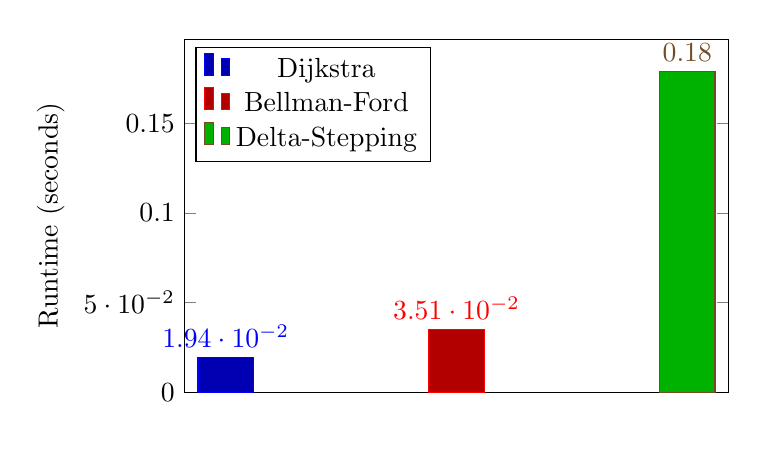
\begin{tikzpicture}
        \begin{axis}[
            ybar,
            bar width=20pt,
            ylabel={Runtime (seconds)},
            symbolic x coords={Dijkstra, Bellman-Ford, Delta-Stepping},
            xtick=data,
            xtick style={draw=none},
            xticklabels={},
            nodes near coords,
            ymin=0,
            width=0.7\textwidth,
            height=0.5\textwidth,
            enlarge x limits=0.3,
            legend style={at={(0.02,0.98)},anchor=north west}
        ]
        \addplot+[ybar, fill=blue!70!black] coordinates {(Dijkstra, 0.0194)};
        \addplot+[ybar, fill=red!70!black] coordinates {(Bellman-Ford, 0.0351)};
        \addplot+[ybar, fill=green!70!black] coordinates {(Delta-Stepping, 0.1788)};
        \legend{Dijkstra, Bellman-Ford, Delta-Stepping}
        \end{axis}
    \end{tikzpicture}
    \caption{Sequential runtime comparison of Dijkstra, Bellman-Ford, and Delta-Stepping algorithms on the \texttt{internet.egr} graph.}
    \label{fig:seq-sssp-times}
\end{figure}

As shown in Figure 1, Dijkstra's algorithm achieved the fastest sequential runtime, followed by Bellman-Ford, with Delta-Stepping being the slowest. 
This ordering is expected, Dijkstra's algorithm is highly efficient for graphs with non-negative edge weights due to its use of a priority queue and greedy selection of the minimum-distance nodes. 
While Bellman-Ford is more flexible in handling negative weights, it incurs additional overhead computation by relaxing all edges in each iteration. 
Although Delta-Stepping is designed for parallel efficiency, it introduces extra overhead in the sequential case from managing buckets and additional data structures, which makes it less efficient than the other two algorithms when run on a single thread. 
These results provide a baseline for evaluating the impact of parallelization in the following sections.

\section{Results and Discussion}

We conducted extensive experiments using all three parallelization frameworks (OpenMP, pthreads, and MPI) with 1, 4, 8, and 16 threads/processes. 
All experiments were performed on the \texttt{internet.egr} graph (124,651 nodes, 387,240 edges) from the DIMACS benchmark suite. 
For Delta-Stepping, we used $\delta = 500$ for all parallel implementations.

\subsection{OpenMP Results}

Table 1 shows the runtime performance of all three algorithms using OpenMP parallelization.

\begin{table}[ht]
\centering
\caption{OpenMP runtime results (seconds) on \texttt{internet.egr}}
\label{tab:omp-results}
\begin{tabular}{lcccc}
\toprule
Algorithm & 1 Thread & 4 Threads & 8 Threads & 16 Threads \\
\midrule
Dijkstra       & 0.0207 & 0.0216 & 0.0216 & 0.0179 \\
Bellman-Ford   & 0.0664 & 0.0324 & 0.0280 & 0.0255 \\
Delta-Stepping & 0.1966 & 0.2814 & 0.3199 & 0.3728 \\
\bottomrule
\end{tabular}
\end{table}

The OpenMP results reveal distinct scalability patterns across the three algorithms. 
\textbf{Dijkstra's algorithm} shows minimal improvement with additional threads, achieving only a modest 13\% speedup from 1 to 16 threads. This limited scalability is expected given Dijkstra's inherently sequential nature. The algorithm requires selecting the global minimum-distance node at each step, creating a serialization bottleneck that prevents effective parallelization. The slight improvement at 16 threads may be attributed to better cache utilization during the initialization phase.

\textbf{Bellman-Ford} demonstrates good scaling behavior, achieving a 2.6× speedup with 16 threads. 
The algorithm's structure, relaxing all edges in parallel during each iteration, is well-suited to OpenMP's work-sharing constructs. 
Our implementation uses atomic operations for thread-safe distance updates, avoiding the overhead of critical sections while maintaining correctness. 
The diminishing returns beyond 8 threads suggest that synchronization costs and memory contention begin to offset the benefits of additional parallelism.

\textbf{Delta-Stepping} exhibits unexpected \textit{negative scaling}, where performance degrades as more threads are added. 
With 16 threads, the algorithm runs 1.9× \textit{slower} than the single-threaded version. 
This counterintuitive result can be attributed to the high synchronization overhead inherent in the bucket-based approach. 
Each bucket processing phase requires a barrier synchronization, and with $\delta = 500$, the algorithm creates frequent synchronization points. 
Additionally, the thread-local bucket merging strategy introduces contention when multiple threads attempt to insert nodes into shared buckets.

\subsection{Pthreads Results}

Table 2 presents the runtime performance using pthreads.

\begin{table}[ht]
\centering
\caption{Pthread runtime results (seconds) on \texttt{internet.egr}}
\label{tab:pthread-results}
\begin{tabular}{lcccc}
\toprule
Algorithm & 1 Thread & 4 Threads & 8 Threads & 16 Threads \\
\midrule
Dijkstra       & 26.65 & 38.54 & 41.48 & 48.91 \\
Bellman-Ford   & 0.0507 & 0.0243 & 0.0122 & 0.0144 \\
Delta-Stepping & 0.240 & 0.208 & 0.199 & 0.223 \\
\bottomrule
\end{tabular}
\end{table}

The pthread results provide interesting insights into low-level thread management. 
\textbf{Dijkstra's pthread implementation} shows severe performance degradation with increasing thread counts, becoming 1.8× slower with 16 threads compared to a single thread. 
This dramatic slowdown is likely due to inefficient parallelization strategy. Our pthread implementation attempts to parallelize the minimum-distance node selection through thread-local searches, but the overhead of thread coordination and the need for global synchronization after each selection far outweighs any computational benefits.

\textbf{Bellman-Ford with pthreads} achieves excellent scalability, showing a 4.2× speedup with 8 threads. 
This is the best scaling result across all implementations and parallelization frameworks. 
The pthread implementation uses a custom work-distribution scheme where each thread processes a contiguous chunk of edges, minimizing false sharing and cache line bouncing. 
The slight performance regression from 8 to 16 threads (0.0122s to 0.0144s) suggests that the computational workload is insufficient to offset thread creation and management costs at higher thread counts.

\textbf{Delta-Stepping with pthreads} performs reasonably well, achieving a 1.2× speedup with 8 threads before experiencing slight degradation at 16 threads. 
The pthread implementation uses thread-local bucket arrays that are merged after each phase, reducing contention compared to the OpenMP version. 
However, the barrier synchronization required between bucket processing phases still limits scalability.

\subsection{MPI Results}

Table 3 shows the runtime performance using MPI parallelization across multiple processes.

\begin{table}[ht]
\centering
\caption{MPI runtime results (seconds) on \texttt{internet.egr}}
\label{tab:mpi-results}
\begin{tabular}{lcccc}
\toprule
Algorithm & 1 Process & 4 Processes & 8 Processes & 16 Processes \\
\midrule
Dijkstra       & 4.97 & 90.82 & 182.91 & 322.70 \\
Bellman-Ford   & 0.0334 & 0.0224 & 0.0246 & 0.0301 \\
Delta-Stepping & 0.296 & 0.738 & 1.966 & 4.319 \\
\bottomrule
\end{tabular}
\end{table}

The MPI results reveal significant challenges with distributed-memory parallelization for these SSSP algorithms. 
\textbf{Dijkstra's MPI implementation} shows catastrophic performance degradation, becoming 65× slower with 16 processes compared to a single process. 
This extreme slowdown is due to the high communication overhead inherent in the distributed implementation. Each process must broadcast its locally-selected minimum node to all other processes at every iteration, and the global minimum selection requires collective communication (MPI\_Allreduce). 
With frequent synchronization points and relatively small computation between communications, the MPI communication latency completely dominates the runtime.

\textbf{Bellman-Ford with MPI} achieves modest speedup with 4 processes (1.5×), demonstrating the best MPI scaling among the three algorithms. 
The edge-relaxation pattern in Bellman-Ford maps naturally to distributed computation, with each process handling a partition of edges. 
However, scaling degrades beyond 4 processes, with 16 processes performing only slightly better than 1 process. 
This degradation is likely due to increased communication overhead as the computation-to-communication ratio becomes unfavorable. Each process has fewer edges to relax, but still must participate in global distance updates and convergence detection.

\textbf{Delta-Stepping with MPI} exhibits severe negative scaling, running 14.6× slower with 16 processes than with 1 process. 
The bucket-based algorithm requires frequent global synchronization to determine which bucket to process next, and the distributed bucket management introduces substantial communication overhead. 
Each process maintains local buckets, but coordinating bucket transitions across processes requires collective operations. 
The highly skewed bucket distribution (98.2\% of nodes in bucket 0) exacerbates this problem, as most processes have little work to do but must still participate in synchronization.

\subsection{Comparative Analysis}

Figure 2 shows the speedup curves for each algorithm across the three parallelization frameworks.

\begin{figure}[ht]
    \centering
    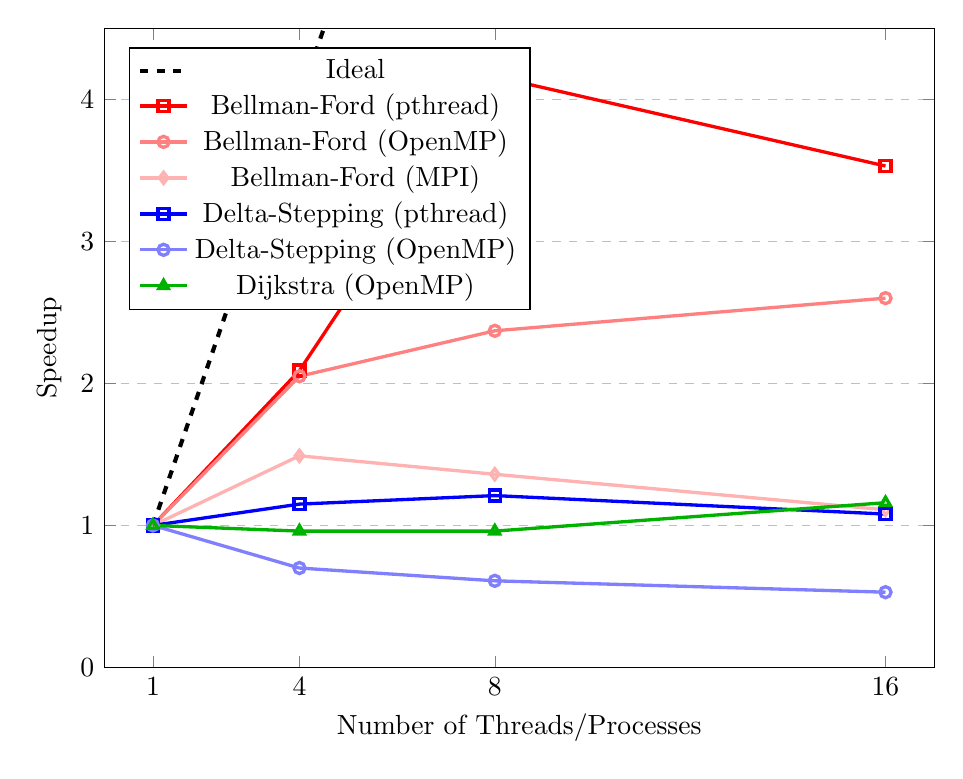
\begin{tikzpicture}
        \begin{axis}[
            xlabel={Number of Threads/Processes},
            ylabel={Speedup},
            xmin=0, xmax=17,
            ymin=0, ymax=4.5,
            xtick={1,4,8,16},
            ytick={0,1,2,3,4},
            legend pos=north west,
            ymajorgrids=true,
            grid style=dashed,
            width=\textwidth,
            height=0.8\textwidth,
        ]
        
        % Ideal speedup
        \addplot[color=black, dashed, line width=1.5pt]
            coordinates {(1,1)(4,4)(8,8)(16,16)};
        \addlegendentry{Ideal}
        
        % Bellman-Ford Pthread
        \addplot[color=red, mark=square, line width=1.2pt]
            coordinates {(1,1)(4,2.09)(8,4.16)(16,3.53)};
        \addlegendentry{Bellman-Ford (pthread)}
        
        % Bellman-Ford OpenMP
        \addplot[color=red!50, mark=o, line width=1.2pt]
            coordinates {(1,1)(4,2.05)(8,2.37)(16,2.60)};
        \addlegendentry{Bellman-Ford (OpenMP)}
        
        % Bellman-Ford MPI
        \addplot[color=red!30, mark=diamond, line width=1.2pt]
            coordinates {(1,1)(4,1.49)(8,1.36)(16,1.11)};
        \addlegendentry{Bellman-Ford (MPI)}
        
        % Delta-Stepping Pthread
        \addplot[color=blue, mark=square, line width=1.2pt]
            coordinates {(1,1)(4,1.15)(8,1.21)(16,1.08)};
        \addlegendentry{Delta-Stepping (pthread)}
        
        % Delta-Stepping OpenMP
        \addplot[color=blue!50, mark=o, line width=1.2pt]
            coordinates {(1,1)(4,0.70)(8,0.61)(16,0.53)};
        \addlegendentry{Delta-Stepping (OpenMP)}
        
        % Dijkstra (both show poor scaling)
        \addplot[color=green!70!black, mark=triangle, line width=1.2pt]
            coordinates {(1,1)(4,0.96)(8,0.96)(16,1.16)};
        \addlegendentry{Dijkstra (OpenMP)}
        
        \end{axis}
    \end{tikzpicture}
    \caption{Speedup comparison across algorithms and parallelization frameworks. Speedup is calculated relative to single-thread/process performance for each implementation.}
    \label{fig:speedup-comparison}
\end{figure}

The comparative analysis reveals several key insights:

\begin{itemize}
    \item \textbf{Algorithm matters more than framework}: Bellman-Ford consistently outperforms Delta-Stepping in terms of scalability, regardless of the parallelization framework used. This suggests that algorithmic structure (edge-centric vs. bucket-based) has a more significant impact on parallel performance than implementation details.
    
    \item \textbf{Shared memory outperforms distributed memory}: The pthread and OpenMP implementations significantly outperform MPI for all algorithms. MPI's communication overhead completely dominates performance, even for relatively communication-efficient algorithms like Bellman-Ford. This indicates that for SSSP on moderately-sized graphs, shared-memory parallelism is strongly preferred over distributed-memory approaches.
    
    \item \textbf{Pthreads provide better control}: The pthread implementations generally achieve better speedups than OpenMP, particularly for Bellman-Ford. This is likely due to more explicit control over thread work distribution and reduced overhead from runtime thread management.
    
    \item \textbf{Delta parameter is critical}: The choice of $\delta = 500$ for Delta-Stepping proved suboptimal for this graph structure. The per-bucket statistics from the pthread implementation (shown in Table 4) reveal that 98.2\% of nodes are finalized in bucket 0, indicating that a much smaller $\delta$ value would provide better load balance and parallelism.
    
    \item \textbf{Synchronization overhead dominates}: For both Dijkstra and Delta-Stepping, the overhead of synchronization (barriers, atomic operations, locks, and especially MPI collective operations) outweighs the computational benefits of parallelization, leading to poor or negative scaling.
\end{itemize}

\begin{table}[ht]
\centering
\caption{Distribution of finalized nodes across Delta-Stepping buckets ($\delta=500$)}
\label{tab:bucket-dist}
\begin{tabular}{ccc}
\toprule
Bucket & Distance Range & Nodes Finalized \\
\midrule
0 & [0, 500)     & 122,363 (98.2\%) \\
1 & [500, 1000)  & 1,694 (1.4\%) \\
2 & [1000, 1500) & 71 (0.1\%) \\
3 & [1500, 2000) & 487 (0.4\%) \\
4 & [2000, 2500) & 28 (0.0\%) \\
5 & [2500, 3000) & 6 (0.0\%) \\
\bottomrule
\end{tabular}
\end{table}

The bucket distribution demonstrates that the graph has a highly skewed distance distribution, with the vast majority of nodes being very close to the source node. 
This property makes it difficult for bucket-based algorithms to expose sufficient parallelism.

\section{Conclusion}

This comparative study evaluated three single-source shortest path algorithms (Dijkstra, Bellman-Ford, and Delta-Stepping) across three parallel programming models: OpenMP, pthreads, and MPI on the DIMACS \texttt{internet.egr} graph (124,651 nodes, 387,240 edges).

Our results demonstrate that algorithm selection dominates framework choice for parallel SSSP performance. 
Bellman-Ford's edge-centric relaxation pattern achieved strong scalability, with a speedup of 4.2 using pthreads and 2.6 using OpenMP, while Dijkstra's inherently sequential structure and Delta-Stepping's synchronization overhead exhibited poor or negative scaling across all frameworks.
Shared-memory parallelism significantly outperformed distributed-memory approaches, with MPI suffering from communication overhead that caused up to a 65-fold slowdown for Dijkstra and a 14.6-fold slowdown for Delta-Stepping.
Pthread implementations generally outperformed OpenMP, particularly for Bellman-Ford, demonstrating the value of explicit thread control for performance-critical applications.

For those working with parallel algorithms, we recommend using Bellman-Ford with pthreads or OpenMP for shared-memory systems, avoiding MPI for single-node deployments, and considering sequential or GPU-accelerated implementations for Dijkstra. 
Parameter tuning proved critical for Delta-Stepping, as our fixed $\delta = 500$ resulted in severe load imbalance (98.2\% of nodes in bucket 0), highlighting the need for adaptive parameter selection.

Future work should explore performance across diverse graph topologies, true distributed-cluster experiments with high-speed interconnects, adaptive $\delta$ selection strategies, and hybrid parallelization approaches combining multiple programming models or GPU acceleration. 
This work demonstrates that effective parallelization requires careful matching of algorithmic structure to parallelization framework, as naive parallelization can degrade rather than improve performance.

\bibliographystyle{unsrtnat}
\bibliography{references}

\end{document}